\section{Speech LLM Data Synthesis}
\label{sec:speechllm_data_synth}

GigaSpeech does not provide translations. We therefore translate transcripts into Chinese/German/Japanese using Qwen3-30B-A3B-Instruct-2507-FP8\footnote{\url{https://huggingface.co/Qwen/Qwen3-30B-A3B-Instruct-2507-FP8}} with prompt \ref{lst:translation_prompt} and filter out low-quality translations with MetricX-QE~\citep{juraska-etal-2024-metricx}\footnote{\url{https://huggingface.co/google/metricx-24-hybrid-xl-v2p6}} by discarding instances with scores below $-3.0$. We subsample 12.5K instances for Speech LLM fine-tuning.


\begin{lstlisting}[
    language=, 
    caption={The prompt template used for synthesizing translation.}, 
    label={lst:translation_prompt}, 
    basicstyle=\ttfamily\footnotesize, 
    breaklines=true, 
    frame=single, 
    columns=fullflexible,
    escapeinside={(*@}{@*)} % <--- 关键设置：定义逃逸符号，允许在代码里插入 LaTeX
]
You are given English document split into lines. Translate each line into Chinese. Do not include any other text.
<begin>
{}
<end>
\end{lstlisting}


\section{Wikidata Utterance Generation Prompt}
\label{app:wiki_utterance_prompt}

The prompt template below is used to elicit term-anchored English utterances for Wikidata-derived retriever training examples. Each batch contains a JSON list of terms and short descriptions, and the model is required to return raw JSON.

\begin{tcolorbox}[
    enhanced,
    breakable,
    colback=gray!3,
    colframe=gray!55!black,
    title={Prompt template for Wikidata term utterance generation},
    fonttitle=\bfseries,
    boxrule=0.4pt,
    arc=1mm,
    left=1.5mm,
    right=1.5mm,
    top=1mm,
    bottom=1mm
]
{\ttfamily\footnotesize
\textbf{System instruction:}\par
You are a dataset builder for speech recognition research.\par
Your task: given a list of terms with their short descriptions, generate short English utterances (5--15 words each) that a speaker might say in a lecture, tutorial, or technical discussion. Use the description as context to produce accurate, meaningful sentences, but do NOT just copy the description.\par
Each utterance MUST contain the given term EXACTLY as written (same spelling, but case may differ). Vary sentence structure and term position (beginning, middle, end). Do NOT repeat the same pattern across terms.\par
Output valid JSON only -- no markdown fences, no explanation.\par
\vspace{0.5em}
\textbf{User prompt:}\par
Generate \{variants\_per\_term\} short utterances (5--15 words) for EACH of the following terms. Use the description as context to make the utterance accurate and meaningful. Each utterance must contain the term verbatim.\par
\vspace{0.5em}
Terms with descriptions:\par
[\par
\hspace*{1em}\{"term": "Seismology", "description": "scientific study of earthquakes"\},\par
\hspace*{1em}\{"term": "dataflow graph", "description": "graph representation of data dependencies"\}\par
]\par
\vspace{0.5em}
Return a JSON object mapping each term to a list of \{variants\_per\_term\} utterance strings. Example format:\par
\{\par
\hspace*{1em}"Seismology": [\par
\hspace*{2em}"Seismology helps us understand earthquake patterns.",\par
\hspace*{2em}"The field of seismology has advanced rapidly."\par
\hspace*{1em}]\par
\}\par
\vspace{0.5em}
IMPORTANT: output raw JSON only, no markdown code fences.\par
}
\end{tcolorbox}


\section{Term Duration Distribution}
\label{app:term_duration}
We show the distribution of term duration on GigaSpeech training set in Figure \ref{fig:term_duration}.

\begin{figure}[h]
    \centering
    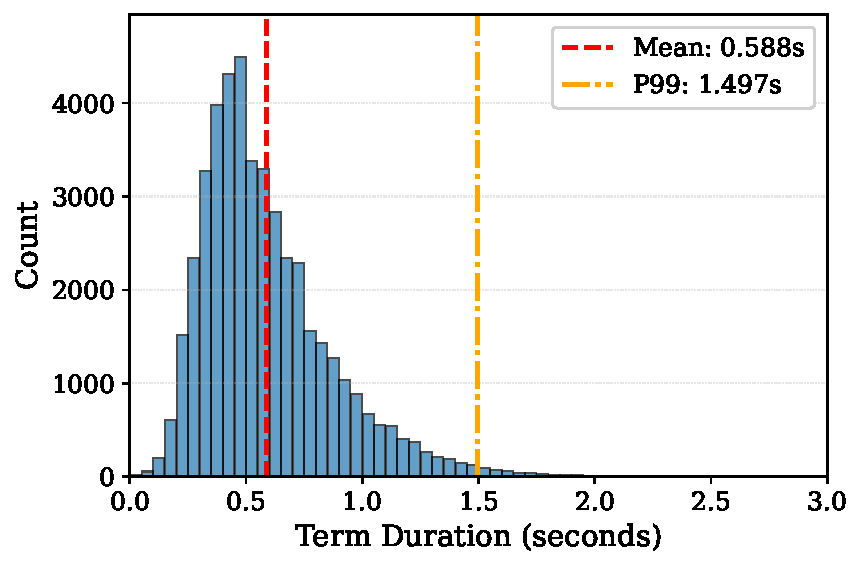
\includegraphics[width=0.7\linewidth]{latex/figures/term_duration_dist.pdf}
    \caption{The distribution of term duration on GigaSpeech training set. }
    \label{fig:term_duration}
\end{figure}

\section{Training Data Prompt Template}
\label{app:prompt_template}

Figure~\ref{fig:train_prompt_visual} illustrates a complete training instance for the SST model.

\definecolor{trainframe}{RGB}{78, 86, 96}
\definecolor{trainsystembg}{RGB}{245, 248, 252}
\definecolor{trainuserbg}{RGB}{247, 250, 246}
\definecolor{trainassistantbg}{RGB}{255, 249, 239}
\providecommand{\appzh}[1]{\begin{CJK*}{UTF8}{gbsn}#1\end{CJK*}}
\newcommand{\trainbox}[2]{%
    \fcolorbox{trainframe}{#1}{%
        \begin{minipage}{\dimexpr\linewidth-2\fboxsep-2\fboxrule\relax}
        #2
        \end{minipage}%
    }%
}

\begin{figure*}[t]
\centering
\begingroup
\setlength{\fboxsep}{5pt}
\setlength{\fboxrule}{0.35pt}
\renewcommand{\arraystretch}{1.08}
\scriptsize
\begin{tabularx}{\textwidth}{@{}>{\bfseries}p{0.12\textwidth}>{\raggedright\arraybackslash}X@{}}
System &
\trainbox{trainsystembg}{You are a professional simultaneous interpreter. You will be given chunks of English audio and you need to translate the audio into Chinese text. Use the \texttt{term\_map} as a reference for terminology if provided.} \\
\addlinespace[0.45ex]
Audio &
\trainbox{trainsystembg}{\texttt{audio\_chunk\_0.wav} \quad $\rightarrow$ \quad \texttt{audio\_chunk\_1.wav} \quad $\rightarrow$ \quad \texttt{audio\_chunk\_2.wav}} \\
\addlinespace[0.45ex]
User 1 &
\trainbox{trainuserbg}{\texttt{\textless audio\textgreater}\par\textbf{term\_map:}
\texttt{things} $\rightarrow$ \appzh{事}; \texttt{everything} $\rightarrow$ \appzh{所有努力}; \texttt{right} $\rightarrow$ \appzh{权利}; \texttt{thing} $\rightarrow$ \appzh{东西}; \texttt{that thing} $\rightarrow$ \appzh{那东西}.} \\
Assistant 1 &
\trainbox{trainassistantbg}{\appzh{她会做些我本意不想让她做的}\texttt{\textless term\textgreater}\appzh{事}\texttt{\textless/term\textgreater}\appzh{。这样一来，之前}\texttt{\textless term\textgreater}\appzh{所有努力}\texttt{\textless/term\textgreater}\appzh{都白费了，我不得不重新写一遍。}} \\
\addlinespace[0.45ex]
User 2 &
\trainbox{trainuserbg}{\texttt{\textless audio\textgreater}\par\textbf{term\_map:}
\texttt{the Porch Gable} $\rightarrow$ \appzh{门廊小屋}; \texttt{story} $\rightarrow$ \appzh{传说}; \texttt{Anne} $\rightarrow$ \appzh{安妮}; \texttt{seclusion} $\rightarrow$ \appzh{静谧}; \texttt{Diana} $\rightarrow$ \appzh{戴安娜}; \texttt{gabelle} $\rightarrow$ \appzh{法国盐税}; \texttt{that story} $\rightarrow$ \appzh{这个故事}; \texttt{porch} $\rightarrow$ \appzh{门廊}.} \\
Assistant 2 &
\trainbox{trainassistantbg}{\appzh{然而，最终}\texttt{\textless term\textgreater}\appzh{传说}\texttt{\textless/term\textgreater}\appzh{终于完成了，}\texttt{\textless term\textgreater}\appzh{安妮}\texttt{\textless/term\textgreater}\appzh{在}\texttt{\textless term\textgreater}\appzh{门廊小屋}\texttt{\textless/term\textgreater}\appzh{的}\texttt{\textless term\textgreater}\appzh{静谧}\texttt{\textless/term\textgreater}\appzh{中把它读给了}\texttt{\textless term\textgreater}\appzh{戴安娜}\texttt{\textless/term\textgreater}\appzh{听。她}} \\
\addlinespace[0.45ex]
User 3 &
\trainbox{trainuserbg}{\texttt{\textless audio\textgreater}\par\textbf{term\_map:}
\texttt{Diana} $\rightarrow$ \appzh{戴安娜}; \texttt{watchful eye} $\rightarrow$ \appzh{密切留意}; \texttt{Robert Ray} $\rightarrow$ \appzh{罗伯特·雷}; \texttt{her pathetic scene} $\rightarrow$ \appzh{那个悲情场景}; \texttt{scene} $\rightarrow$ \appzh{现场}; \texttt{that scene} $\rightarrow$ \appzh{那场戏}.} \\
Assistant 3 &
\trainbox{trainassistantbg}{\appzh{成功地呈现了那个悲情场景，同时又没有牺牲}\texttt{\textless term\textgreater}\appzh{罗伯特·雷}\texttt{\textless/term\textgreater}\appzh{，她一边读一边}\texttt{\textless term\textgreater}\appzh{密切留意}\texttt{\textless/term\textgreater}\appzh{着}\texttt{\textless term\textgreater}\appzh{戴安娜}\texttt{\textless/term\textgreater}\appzh{的反应。戴安娜}} \\
\end{tabularx}
\endgroup
\caption{A visualized Chinese new\_v10 training sample. Each user turn supplies one audio chunk and a retrieved term map; the assistant target is the corresponding partial translation with supervised term tags.}
\label{fig:train_prompt_visual}
\end{figure*}


\section{Glossary Extraction Details}
\label{app:glossary_extraction}

To simulate a realistic deployment scenario, we extract a glossary from the reference paper PDFs using \texttt{Gemini-2.5-Flash}\footnote{\url{https://docs.cloud.google.com/vertex-ai/generative-ai/docs/models/gemini/2-5-flash}}. 



\subsection{Prompting Strategy}
We feed the full text of each paper into the model and use a structured prompt to identify domain-specific terms, acronyms, and their corresponding translations in Chinese, German, and Japanese. The exact prompt template is provided in Listing~\ref{lst:extraction_prompt}.
To ensure robustness, we re-prompts the model to fix malformed JSON outputs if parsing fails. 
Finally, we deduplicate terms within each paper using case-insensitive matching. 


\begin{lstlisting}[
    language=, 
    caption={The prompt template used for terminology extraction and translation.}, 
    label={lst:extraction_prompt}, 
    basicstyle=\ttfamily\footnotesize, 
    breaklines=true, 
    frame=single, 
    columns=fullflexible,
    escapeinside={(*@}{@*)} % <--- 关键：定义逃逸符号，允许在代码里插入 LaTeX
]
Extract technical glossary terms from the following ACL paper text and provide translations.

Focus on:
- Domain-specific terms (NLP / speech / ML)
- Terms likely mentioned in oral presentations
- Substantive technical concepts (not common words)
- Acronyms

For each term, provide:
1. The term itself (in English)
2. Translations in Chinese (zh), German (de), and Japanese (ja)

Return ONLY a valid JSON array (no markdown, no commentary). Format:
[
  {
    "term": "BERT",
    "target_translations": {
      "zh": "BERT",
      "de": "BERT",
      "ja": "BERT"
    }
  },
  {
    "term": "attention mechanism",
    "target_translations": {
      "zh": "(*@\begin{CJK*}{UTF8}{gbsn}注意力机制\end{CJK*}@*)",
      "de": "Aufmerksamkeitsmechanismus",
      "ja": "(*@\begin{CJK*}{UTF8}{min}注意機構\end{CJK*}@*)"
    }
  }
]

Constraints:
- Extract as many relevant technical terms as you can.
- Do not include author names, affiliations, or generic phrases.
- If the same term appears multiple times, list it only once.
- For acronyms, provide the acronym itself (not the full form).

PAPER_TEXT:
__PAPER_TEXT__

Return ONLY the JSON array, nothing else.
\end{lstlisting}

\subsection{Extraction Examples}
Table~\ref{tab:extracted_examples} shows a subset of terms automatically extracted from the paper \textit{"Online Semantic Parsing for Latency Reduction in Task-Oriented Dialogue"} (2022.acl-long.110). The model successfully identifies specific acronyms (e.g., FLR, SimulMT) and technical concepts (e.g., online semantic parsing).

\begin{table*}[h]
\centering
\small
\begin{tabular}{l|p{9cm}}
\toprule
\textbf{Extracted Term} & \textbf{Target Translations (Zh / De / Ja)} \\
\midrule
online semantic parsing & \textbf{Zh}: \begin{CJK*}{UTF8}{gbsn}在线语义解析\end{CJK*}; \textbf{De}: Online-Semantikparsing; \textbf{Ja}: \begin{CJK*}{UTF8}{min}オンライン意味解析\end{CJK*} \\
\midrule
FLR & \textbf{Zh}: \begin{CJK*}{UTF8}{gbsn}最终延迟减少\end{CJK*}; \textbf{De}: Endlatenzreduzierung; \textbf{Ja}: \begin{CJK*}{UTF8}{min}最終レイテンシ削減\end{CJK*} \\
\midrule
SimulMT & \textbf{Zh}: \begin{CJK*}{UTF8}{gbsn}同声机器翻译\end{CJK*}; \textbf{De}: Simultane MÜ; \textbf{Ja}: \begin{CJK*}{UTF8}{min}同時機械翻訳\end{CJK*} \\
\midrule
ASR & \textbf{Zh}: \begin{CJK*}{UTF8}{gbsn}自动语音识别\end{CJK*}; \textbf{De}: Automatische Spracherkennung; \textbf{Ja}: \begin{CJK*}{UTF8}{min}自動音声認識\end{CJK*} \\
\midrule
dataflow graph & \textbf{Zh}: \begin{CJK*}{UTF8}{gbsn}数据流图\end{CJK*}; \textbf{De}: Datenflussgraph; \textbf{Ja}: \begin{CJK*}{UTF8}{min}データフローグラフ\end{CJK*} \\
\midrule
PREFIXTOGRAPH & \textbf{Zh}: PREFIXTOGRAPH; \textbf{De}: PREFIXTOGRAPH; \textbf{Ja}: PREFIXTOGRAPH \\
\bottomrule
\end{tabular}
\caption{Examples of extracted terms and their multilingual translations from paper 2022.acl-long.110. Note that acronyms or specific model names (e.g., PREFIXTOGRAPH) are often preserved in target languages.}
\label{tab:extracted_examples}
\end{table*}

\section{Runtime Glossary-Bank Ablation Details}
\label{app:glossary_bank_ablation}

Table~\ref{tab:app_glossary_bank_ablation_full} reports the complete En-Zh runtime glossary-bank ablation. The main text plots only the ACL tagged rows to keep the ablation compact. We include the medicine rows here as a stricter curated-domain stress test: the denominator is manually verified and intentionally targets specialized clinical terms and exact target forms that are difficult for streaming systems. The rows use the same fixed raw-denominator scoring rule, but the larger expanded banks contain more near-duplicate and variant translations, which can reduce exact TERM\_ACC even when BLEU remains stable.

\begin{table*}[t]
\centering
\small
\resizebox{\linewidth}{!}{%
\begin{tabular}{llrrrrrr}
\toprule
Dataset & Bank & LM & BLEU & StreamLAAL & TERM\_ACC & RealAdopt & FCR \\
\midrule
Tagged ACL & raw & 1 & 44.41 & 1237 & 85.39 & 89.40 & 13.01 \\
 & raw & 2 & 49.61 & 1862 & 88.88 & 90.37 & 12.41 \\
 & raw & 3 & 50.15 & 2343 & 89.89 & 91.08 & 8.07 \\
 & raw & 4 & 50.81 & 2786 & 90.00 & 92.12 & 9.40 \\
 & gs1k & 1 & 46.92 & 1320 & 86.29 & 89.84 & 10.32 \\
 & gs1k & 2 & 48.74 & 1927 & 89.10 & 90.48 & 12.76 \\
 & gs1k & 3 & 49.82 & 2427 & 88.09 & 89.99 & 7.95 \\
 & gs1k & 4 & 50.23 & 2824 & 89.10 & 91.36 & 9.33 \\
 & gs10k & 1 & 46.20 & 1373 & 84.61 & 88.11 & 9.38 \\
 & gs10k & 2 & 49.07 & 1913 & 88.54 & 90.29 & 8.87 \\
 & gs10k & 3 & 49.86 & 2427 & 88.99 & 91.25 & 8.32 \\
 & gs10k & 4 & 50.35 & 2828 & 88.65 & 91.37 & 10.28 \\
\midrule
Medicine & raw & 1 & 33.40 & 1140 & 79.05 & 84.23 & 30.79 \\
 & raw & 2 & 41.28 & 1772 & 83.36 & 90.52 & 27.51 \\
 & raw & 3 & 43.06 & 2321 & 84.70 & 91.26 & 27.27 \\
 & raw & 4 & 44.36 & 2822 & 85.14 & 92.15 & 25.96 \\
 & gs1k & 1 & 36.37 & 1293 & 75.19 & 85.66 & 30.07 \\
 & gs1k & 2 & 42.11 & 1874 & 78.45 & 87.66 & 23.27 \\
 & gs1k & 3 & 43.42 & 2318 & 80.83 & 90.34 & 20.79 \\
 & gs1k & 4 & 44.40 & 2829 & 81.58 & 90.82 & 20.06 \\
 & gs10k & 1 & 35.92 & 1221 & 74.59 & 84.82 & 28.45 \\
 & gs10k & 2 & 42.02 & 1862 & 78.16 & 88.17 & 22.07 \\
 & gs10k & 3 & 43.34 & 2335 & 80.39 & 89.29 & 18.77 \\
 & gs10k & 4 & 44.10 & 2837 & 79.94 & 88.63 & 17.81 \\
\bottomrule
\end{tabular}%
}
\caption{Full En-Zh runtime glossary-bank ablation. The runtime bank changes from the raw task glossary to GS-1k or GS-10k, while all terminology metrics use the corresponding fixed raw denominator. The main text plots the ACL rows; medicine rows are included as a stricter domain stress test.}
\label{tab:app_glossary_bank_ablation_full}
\end{table*}


\section{Training Details}\label{app:training_details}

\textbf{Retriever.}
We train the retriever with LoRA applied to both the speech and text encoders.
For the audio encoder, LoRA is inserted into the query/key/value/output projections and MLP blocks with rank $r{=}32$ and scaling factor $\alpha{=}64$.
For the text encoder, LoRA targets the query/key/value projections with rank $r{=}16$ and $\alpha{=}32$.
We train with a multi-positive InfoNCE objective using a fixed temperature $\tau{=}0.03$.
We optimize with AdamW (learning rate $1\times10^{-4}$, weight decay 0.01), cosine annealing with 10\% warmup, and gradient clipping (max norm 1.0) under BF16 mixed precision.
